\documentclass[titlepage]{article}

\usepackage[utf8]{inputenc}
\usepackage{scrextend}
\usepackage[bottom]{footmisc}
\usepackage{graphicx}

\title{Comfy: Gestionnaire de fenêtres en tuile}
\author{Daniel-Junior Dubé et Félix Chabot}
\date{Session d'automne 2018}

\graphicspath{ {./images/} }

\begin{document}
    \maketitle

    \renewcommand{\contentsname}{Table des matières}
    \tableofcontents
    \newpage

    \section{Introduction}
    \par
	Étant devenu depuis quelques années des enthousiastes des systèmes d'exploi-tation GNU/Linux, nous avons pu observer l’engouement de la communauté envers les gestionnaires des fenêtre en tuile\footnote{https://en.wikipedia.org/w/index.php?title=Tiling\_window\_manager}. En effet, ces gestionnaires permettent une plus grande flexibilité pour la personnalisation de l’interface utilisateur que les environnements de bureau populaire tel que \textit{Gnome}, \textit{KDE} et \textit{Xfce} tout en étant plus léger sur l’utilisation des ressources matérielles. Tout comme les outils minimalistes tel \textit{Vim} et \textit{Emacs}, ces gestionnaires de fenêtres permettre aussi de bénéficier à l’efficacité des développeurs qui les utilisent grâce aux fonctionnalités adaptées à ceux-ci.

    \par
    \bigskip
    De plus, le tout nouveau protocole \textit{Wayland} commence à être adopté par ces environnements de bureau. Il risque de remplacer le protocole \textit{X} d'ici quelques années à cause de son architecture optimisée et pour sa meilleure gestion des ressources matérielles.

    \par
    \bigskip
	Nous avons donc décidé de concevoir un gestionnaire de fenêtres utilisant ce nouveau protocole et qui sera écrit avec le langage de programmation \textit{Rust}. Celui-ci est un langage apportant des fonctionnalités modernes intéressantes en ce qui concerne la gestion mémoire et la concurrence, tout en gardant une performance rivalisant celle du \textit{C} et \textit{C++}. Il existe peu de gestionnaires de fenêtres utilisant à la fois \textit{Rust} et \textit{Wayland}. Il y en a un en particulier s’appelant \textit{Way-Cooler}\footnote{http://way-cooler.org}, mais selon les auteurs de ce projet, il n’est pas encore assez stable pour être utilisé en “production”.

    \par
    \bigskip
    Notre but sera donc de créer un logiciel que des enthousiastes pourront ultimement utiliser dans leur quotidien tout en nous permettant d’apprendre les rudiments de la programmation de composantes systèmes.

	\section{Revue de littérature}
	\begin{description}
		\item [Écran] Un écran est un espace de rendu qui est mis à notre disposition par un appareil physique (moniteur).
		\item [Espace de travail] Un écran possède une liste d’espaces de travail. Un seul espace de travail est affiché à l’écran à la fois.
		\item [Disposition] Un espace de travail est constitué d’une seule disposition. Celle-ci est sous forme d’un arbre enraciné (k-ary tree), elle va déterminer la position et la dimension des fenêtres.
		\item [Noeud de disposition (dans l’arbre de disposition)] Noeud dans l’arbre de la disposition. Correspond essentiellement à un conteneur de fenêtres.
		\item [Subdivision] Une subdivision représente à la fois une entrée dans l’arbre de disposition et un sous-ensemble de l’espace d’affichage de l’écran.
		\item [Fenêtre] Une fenêtre est une feuille dans l’arbre de disposition. Elle est donc l’espace réservé à l’affichage du rendu d’une application en exécution.
		\item [Conteneur de fenêtres] Un conteneur est un noeud dans l’arbre de disposition. Il s’agit donc d’une structure de données qui va contenir un ensemble de fenêtres ou de conteneurs.
		\item [Gestionnaire de fenêtre] Un logiciel qui contrôle l’affichage et la disposition des fenêtres des applications en exécution.
		\item [Tuile] Correspond à l’espace (ou subdivision) de l’écran réservé à une fenêtre ou un conteneur de fenêtres.
    \end{description}
	
	\section{Diagrammes du fonctionnement}
	\begin{figure}[h]
		\centering
		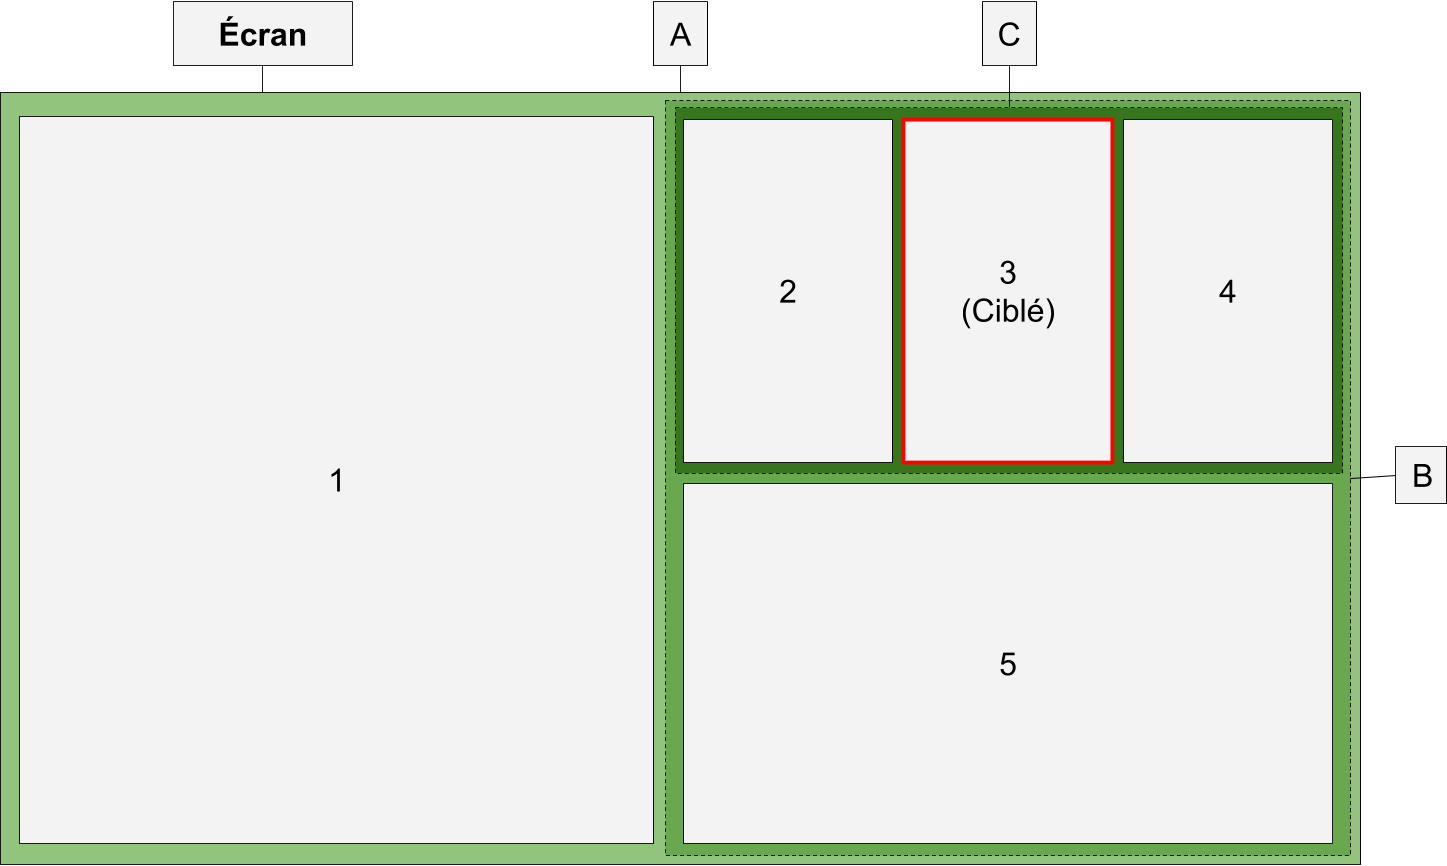
\includegraphics[width=\textwidth]{diagramme_du_fonctionnement.png}
		\caption {Représentation d'une intéraction normale de ces objets}
	\end{figure}
	\begin{figure}[h]
		\centering
		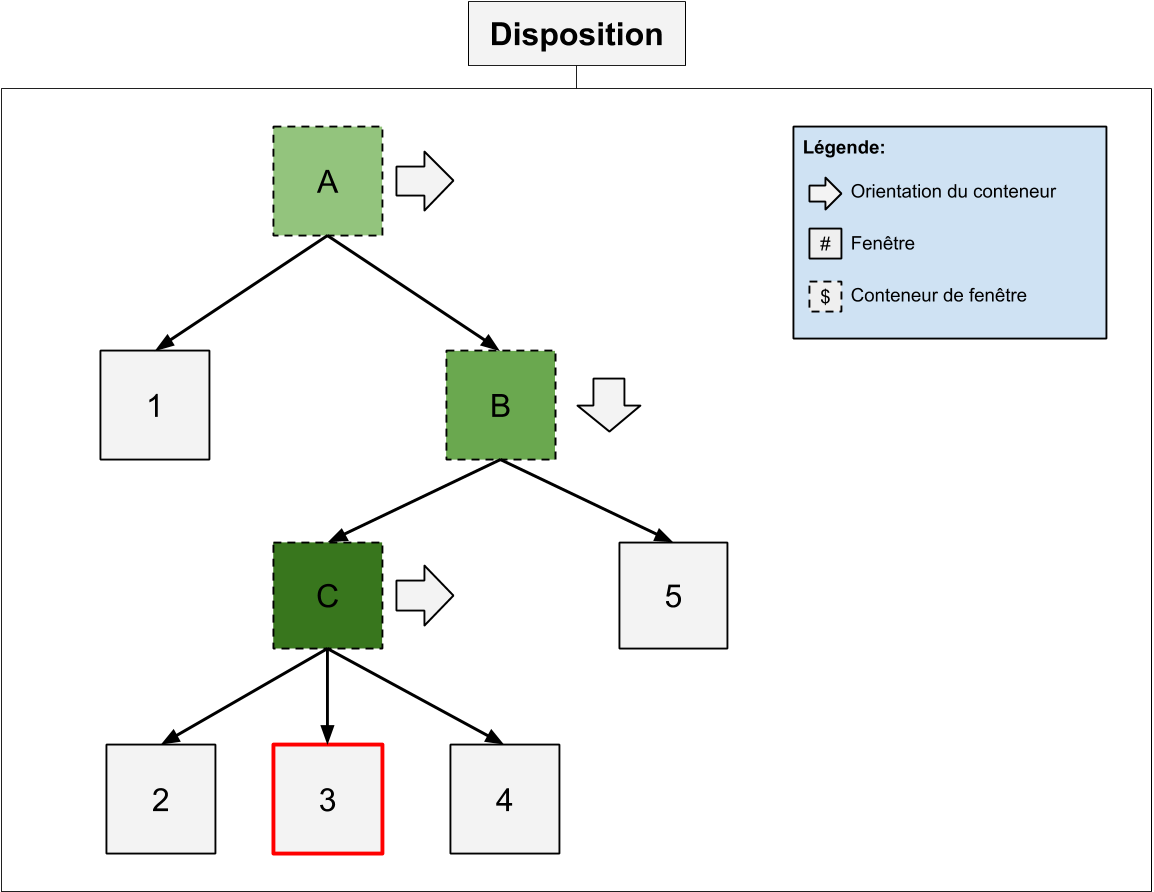
\includegraphics[width=\textwidth]{diagramme_du_fonctionnement_arbre.png}
		\caption {Arbre résultant}
	\end{figure}
\end{document}
